\chapter{Farey Series Approximation}
\label{crla1}

It is often necessary in microcontroller work to approximate
the function

\begin{equation}
\label{eq:crla1:01}
f(x) = r_I x,
\end{equation}

\noindent{}where $r_I \in \vworkrealsetnonneg$ and $f(x), x \in \vworkintsetnonneg$.

This approximation is often made by selecting $r_A = h/k \approx r_I$ and implementing
the approximation as

\begin{equation}
\label{eq:crla1:02}
g(x) = \left\lfloor \frac{hx}{k} \right\rfloor ,
\end{equation}

\noindent{}where $h \in \vworkintsetnonneg$ and $k \in \vworkintsetpos$.

In nearly all cases, it is most efficient to choose $k$ to be power of 2,
so that the approximation can be made with an integer multiplication
followed by a right shift.

However, in rare cases, the approximation can be made as efficiently or
more efficiently with an integer multiplication followed by an integer
division, removing the constraint that $k$ be a power of 2.  This leads to
the question of how to choose $r_A=h/k$ as close as possible to $r_I \in
\vworkrealsetnonneg$, under the constraints that $h \leq h_{MAX}$ and $k
\leq k_{MAX}$.

With the typical constraint that $h \leq h_{MAX} = 2^{32}-1$ and $k \leq
k_{MAX} = 2^{32}-1$, a best rational approximation can be found in a
matter of seconds using an $O(n)$ algorithm.  However, with $h_{MAX} =
k_{MAX} = 2^{64}-1$ (or larger), a best rational approximation can't be
found using an $O(n)$ algorithm in a practical time.

The arrangement of rational numbers is a weighty topic from number theory,
and finding a best rational approximation with large $h_{MAX}$ and
$k_{MAX}$ is a counterintuitively hard problem.  This chapter presents an
$O(log\;n)$ algorithm that can be used to find the best rational
approximation $r_A = h/k$ to an $r_I$ with arbitrarily large $h_{MAX}$ and
$k_{MAX}$.


%%%%%%%%%%%%%%%%%%%%%%%%%%%%%%%%%%%%%%%%%%%%%%%%%%%%%%%%%%%%%%%%%%%%%%%%%%%%%%%
%%%%%%%%%%%%%%%%%%%%%%%%%%%%%%%%%%%%%%%%%%%%%%%%%%%%%%%%%%%%%%%%%%%%%%%%%%%%%%%
%%%%%%%%%%%%%%%%%%%%%%%%%%%%%%%%%%%%%%%%%%%%%%%%%%%%%%%%%%%%%%%%%%%%%%%%%%%%%%%
\section{The Farey Series}
\label{crla1:sfry0}

The \index{Farey series}\emph{Farey}\footnote{Named after geologist John
Farey, whose letter about these series was published in
\emph{Philosophical Magazine} in 1816.} \emph{series of order
$N$},\index{Farey series} denoted $F_{N}$,\index{F@$F_N$} is the ordered
set of all irreducible rational numbers $h/k$ in the interval [0,1] with
denominator $k\leq N$.  As examples, the Farey series of orders 1 through
7, $F_1$ through $F_7$, are shown in (\ref{eq:crla1:sfry0:eq0001a})
through (\ref{eq:crla1:sfry0:eq0001g}).

\begin{equation}
\label{eq:crla1:sfry0:eq0001a}
F_1  = \left\{ {\frac{0}{1},\frac{1}{1}} \right\}
\end{equation}

\begin{equation}
\label{eq:crla1:sfry0:eq0001b}
F_2  = \left\{ {\frac{0}{1},\frac{1}{2},\frac{1}{1}} \right\}
\end{equation}

\begin{equation}
\label{eq:crla1:sfry0:eq0001c}
F_3  = \left\{ {\frac{0}{1},\frac{1}{3},\frac{1}{2},
                \frac{2}{3},\frac{1}{1}} \right\}
\end{equation}

\begin{equation}
\label{eq:crla1:sfry0:eq0001d}
F_4  = \left\{ {\frac{0}{1},\frac{1}{4},
                \frac{1}{3},\frac{1}{2},
                \frac{2}{3},\frac{3}{4},
                \frac{1}{1}} \right\}
\end{equation}

\begin{equation}
\label{eq:crla1:sfry0:eq0001e}
F_5  = \left\{ {\frac{0}{1},\frac{1}{5},\frac{1}{4},
                \frac{1}{3},\frac{2}{5},\frac{1}{2},
                \frac{3}{5},\frac{2}{3},\frac{3}{4},
                \frac{4}{5},\frac{1}{1}} \right\}
\end{equation}

\begin{equation}
\label{eq:crla1:sfry0:eq0001f}
F_6  = \left\{ {\frac{0}{1},\frac{1}{6},\frac{1}{5},
                \frac{1}{4},
                \frac{1}{3},\frac{2}{5},\frac{1}{2},
                \frac{3}{5},\frac{2}{3},
                \frac{3}{4},
                \frac{4}{5},
                \frac{5}{6},\frac{1}{1}} \right\}
\end{equation}


\begin{equation}
\label{eq:crla1:sfry0:eq0001g}
F_7  = \left\{ {\frac{0}{1},\frac{1}{7},\frac{1}{6},\frac{1}{5},
                \frac{1}{4},\frac{2}{7},
                \frac{1}{3},\frac{2}{5},\frac{3}{7},\frac{1}{2},
                \frac{4}{7},\frac{3}{5},\frac{2}{3},
                \frac{5}{7},\frac{3}{4},
                \frac{4}{5},
                \frac{5}{6},\frac{6}{7},\frac{1}{1} } \right\}
\end{equation}

The distribution of Farey rational numbers in [0,1] is repeated in any
$[i,i+1]$, $i\in \vworkintset$; so that the distribution of Farey
rationals in [0,1] supplies complete information about the distribution in
all of $\vworkrealset$\@.  I occasionally abuse the proper nomenclature by
referring to sequential rational numbers outside the interval [0,1] as
Farey terms or as part of $F_N$, which, technically, they are not.  All of
the results presented in this chapter can be shown to apply everywhere in
$\vworkrealsetnonneg$, so this abuse is not harmful.

It can be proved that if $h/k$ is irreducible, then $(h+ik)/k$ is also
irreducible (i.e.  the analogous terms in $[i, i+1]$ corresponding to the
Farey terms in $[0,1]$ are also irreducible).

Recursive formulas exist for generating successive terms of the Farey
series.  Given two successive terms of a Farey series of order $N$,
$h_{j-2}/k_{j-2}$ and $h_{j-1}/k_{j-1}$, (\ref{eq:crla1:sfry0:thm:01:eq01})
and (\ref{eq:crla1:sfry0:thm:01:eq02}) can be applied to generate the next
term, $h_{j}/k_{j}$\@.  In applying (\ref{eq:crla1:sfry0:thm:01:eq01}) and
(\ref{eq:crla1:sfry0:thm:01:eq02}), the two terms used as input must be
irreducible.

\begin{equation}
\label{eq:crla1:sfry0:thm:01:eq01}
h_{j}  = \left\lfloor {\frac{{k_{j-2}
     + N}}{{k_{j - 1} }}} \right\rfloor h_{j - 1}  - h_{j-2}
\end{equation}

\begin{equation}
\label{eq:crla1:sfry0:thm:01:eq02}
k_{j}  = \left\lfloor {\frac{{k_{j-2}  + N}}{{k_{j
     - 1} }}} \right\rfloor k_{j - 1}  - k_{j-2}
\end{equation}

Similarly, given two successive terms of a Farey series of order $N$,
$h_{j+1}/k_{j+1}$ and $h_{j+2}/k_{j+2}$, (\ref{eq:crla1:sfry0:thm:01:eq03})
and (\ref{eq:crla1:sfry0:thm:01:eq04}) can be applied to generate the
preceding term, $h_{j}/k_{j}$\@.  Again, in applying
(\ref{eq:crla1:sfry0:thm:01:eq03}) and (\ref{eq:crla1:sfry0:thm:01:eq04}),
the two terms used as input must be irreducible.

\begin{equation}
\label{eq:crla1:sfry0:thm:01:eq03}
h_j  = \left\lfloor {\frac{{k_{j + 2}  + N}}{{k_{j + 1} }}}
\right\rfloor h_{j + 1}  - h_{j + 2}
\end{equation}

\begin{equation}
\label{eq:crla1:sfry0:thm:01:eq04}
k_j  = \left\lfloor {\frac{{k_{j + 2}  + N}}{{k_{j + 1} }}}
\right\rfloor k_{j + 1}  - k_{j + 2}
\end{equation}

It might appear that (\ref{eq:crla1:sfry0:thm:01:eq01}) through
(\ref{eq:crla1:sfry0:thm:01:eq04}) provide a viable method for finding
best rational approximations (i.e.  start with $0/1$ and $1/N$ and
generate successive terms in $F_N$ until $r_I$ is bracketed), but in fact
they do not.  The number of terms in the Farey series is approximately
quadratic with respect to the order of the series, so generating terms
starting at an integer boundary is $O(N^2)$ and doesn't scale up well for
finding best rational approximations for processors that can operate on
32- and 64-bit integers.

The Farey series has an intuitive graphical interpretation involving the
\index{integer lattice}\index{Farey series!integer lattice
interpretation}integer lattice.  This interpretation is shown in Fig.
\ref{fig:crla1:sfry0:00} (although in the figure, $h$ is also restricted).

\begin{figure}
\centering
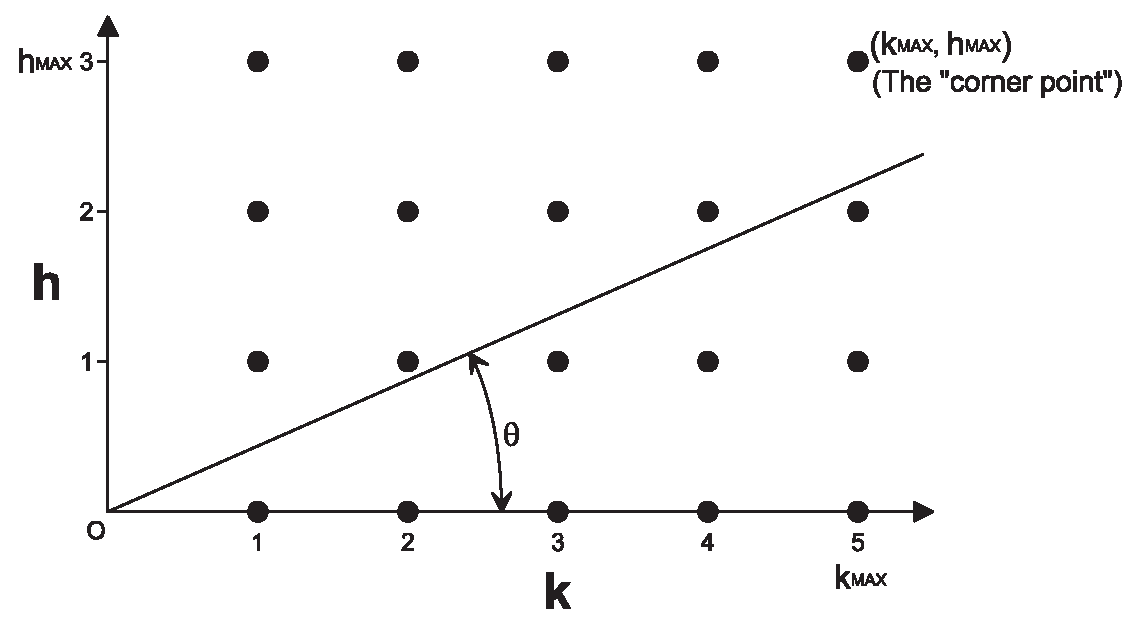
\includegraphics[width=4.6in]{c_rla1/farey01a.eps}
\caption{Graphical Interpretation Of Rational Numbers
         $h/k$ That Can Be Formed With $h \leq h_{MAX}=3$, $k \leq k_{MAX}=5$}
\label{fig:crla1:sfry0:00}
\end{figure}

From the graphical interpretation suggested by Fig.
\ref{fig:crla1:sfry0:00}, the following properties are apparent:

\begin{itemize}
\item The angle of a ray drawn from the origin to the point $(k,h)$
      corresponding to the rational number $h/k$ is $\theta = tan^{-1} \; h/k$.
\item Any integer lattice point on a line from the origin drawn at the
      angle $\theta$ has the value $h/k = tan \; \theta$.  All points
      corresponding to rational numbers with the same value will be on this
      line.
\item A rational number $h/k$ is irreducible if and only if its
      corresponding point $(k,h)$ is directly visible from the origin with
      no intervening points.
\item The Farey series of order $N$, $F_N$, can be formed graphically by
      starting with the set of integer lattice points $(k,h): \; h \in
      \vworkintsetnonneg \wedge 1 \leq k \leq N$, then sweeping a line extended
      from the origin, starting with angle $\theta = 0$, through $0 \leq \theta
      < \pi{}/2$, and recording in order each point directly visible from the
      origin.\footnote{Note that Fig.  \ref{fig:crla1:sfry0:00}, because
      it illustrates the case when $h$ is constrained as well, does not show
      integer lattice points for $h > h_{MAX}$.  If the integer
      lattice shown in Fig.  \ref{fig:crla1:sfry0:00} were extended
      upward, every positive irreducible rational number with
      $k \leq k_{MAX} = 5$ could be found graphically.}
\end{itemize}

Fig.  \ref{fig:crla1:sfry0:01} illustrates the graphical construction
method for $F_5$.  Note that only integer lattice points which are
directly visible from the origin (with no intervening points) are
selected.  (Fig.  \ref{fig:crla1:sfry0:01}, like Fig.
\ref{fig:crla1:sfry0:00}, shows the case of constrained $h$---the integer
lattice should be continued upward to construct $F_5$.)

\begin{figure}
\centering
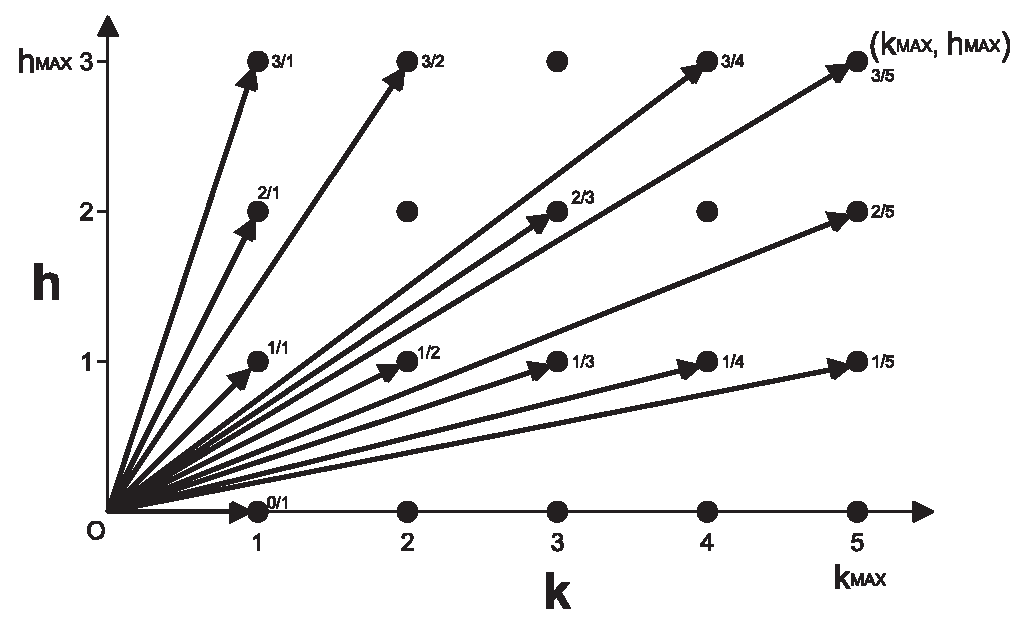
\includegraphics[width=4.6in]{c_rla1/farey01b.eps}
\caption{Graphical Interpretation Of Irreducible Rational Numbers
         $h/k$ That Can Be Formed With $h \leq h_{MAX}=3$, $k \leq k_{MAX}=5$}
\label{fig:crla1:sfry0:01}
\end{figure}

I denote the set of non-negative irreducible rational numbers that can be formed
with $h \leq h_{MAX}$ and $k \leq k_{MAX}$ as $F_{k_{MAX}, h_{MAX}}$\@.
Using this notation, the graphical construction method
depicted in Figure \ref{fig:crla1:sfry0:01} identifies $F_{5,3}$:

\begin{equation}
\label{eq:crla1:sfry0:eq0002a}
F_{5,3}  = \left\{ {\frac{0}{1},\frac{1}{5},\frac{1}{4},
                    \frac{1}{3},\frac{2}{5},\frac{1}{2},
                    \frac{3}{5},\frac{2}{3},\frac{3}{4},
                    \frac{1}{1},\frac{3}{2},\frac{2}{1},
                    \frac{3}{1}} \right\} .
\end{equation}


The ``corner point'' in Figures \ref{fig:crla1:sfry0:00}
and \ref{fig:crla1:sfry0:01}, $k_{MAX}/h_{MAX} = 5/3$, plays a special role:

\begin{itemize}
\item From 0/1 up through the corner point $h_{MAX}/k_{MAX}$,
      the terms are the terms of the Farey series of order
      $k_{MAX}$.
\item From $h_{MAX}/k_{MAX}$ up through $h_{MAX}/1$, the terms
      are the reverse-ordered reciprocals of the terms of the
      Farey series of order $h_{MAX}$\@. (This can be seen
      by transposing the $h$ and $k$ axes of the figures.)
\end{itemize}

The observation about the terms of $F_{5,3}$ that are greater than 3/5 is
important, because it means that if there is a method for finding the
nearest Farey series neighbors to a real number $r_I$ (the case of
only $k$ constrained, $k \leq k_{MAX}$), then there is also a method for finding
the nearest neighbors in $F_{k_{MAX}, h_{MAX}}$ (both $h$ and $k$ constrained).
The method is:

\begin{itemize}
\item If $r_I < k_{MAX}/h_{MAX}$, find the nearest neighbors to $r_I$ in
      $F_{k_{MAX}}$.
\item If $r_I > k_{MAX}/h_{MAX}$, find the nearest neighbors to $1/r_I$
      in $F_{h_{MAX}}$; the reciprocals of those neighbors are the closest
      rational numbers in $F_{k_{MAX}, h_{MAX}}$ to $r_I$.
\end{itemize}

%%%%%%%%%%%%%%%%%%%%%%%%%%%%%%%%%%%%%%%%%%%%%%%%%%%%%%%%%%%%%%%%%%%%%%%%%%%%%%%
%%%%%%%%%%%%%%%%%%%%%%%%%%%%%%%%%%%%%%%%%%%%%%%%%%%%%%%%%%%%%%%%%%%%%%%%%%%%%%%
%%%%%%%%%%%%%%%%%%%%%%%%%%%%%%%%%%%%%%%%%%%%%%%%%%%%%%%%%%%%%%%%%%%%%%%%%%%%%%%
\section{The Continued Fraction Algorithm}
\label{crla1:scfr0}

A \emph{finite simple continued fraction} is a fraction of the form

\begin{equation}
\label{eq:crla1:scfr0:00}
a_0 + \cfrac{1}{a_1 + \cfrac{1}{a_2
    + \cfrac{1}{\;\;\;\;\;\;\;\;\;\;\;\;\;\;\ldots + \cfrac{1}{a_n}}}}
    =
    [a_0; a_1, a_2, \ldots , a_n] ,
\end{equation}

\noindent{}where $a_0 \in \vworkintsetnonneg$ and $a_i \in
\vworkintsetpos$, $i > 0$.  Each integer $a_i$ is called an
\index{continued fraction!element}\emph{element} or \index{continued
fraction!partial quotient}\emph{partial quotient} of the continued
fraction.  To ensure a unique representation, it is required, except in
the case of the continued fraction representation of an integer, that the
final element $a_n$ not be equal to 1.

Continued fractions are unwieldly to write and typeset, so a continued
fraction in the form of (\ref{eq:crla1:scfr0:00}) is written as
$[a_0; a_1, a_2, \ldots , a_n]$.  The separator between $a_0$ and $a_1$ is
a semicolon (`;'), and all other separators are commas (`,').

Continued fractions can be either finite or infinite:

\begin{itemize}
\item A finite continued fraction consists of a finite number of elements
      $[a_0;$ $a_1,$ $a_2,$ $\ldots ,$ $a_n]$\@.  It can be proved that every rational
      number corresponds to a unique finite continued fraction, and that
      every finite continued fraction corresponds to a unique rational number.
\item An infinite continued fraction consists of an infinite number of
      elements $[a_0; a_1, a_2, \ldots]$.  Because every rational number
      corresponds to a finite continued fraction, all irrational numbers have
      infinite continued fraction representations.
\end{itemize}

In engineering work (and due to the general prevalence of computers
and calculators), any $r_I$ to be approximated has a known approximate
numerical value.  Even quantities that are known to be irrational (such
as $\pi$ or $\sqrt{2}$) have a numerical value known to a large number
of significant digits.  For this reason, only the numerical procedure for
obtaining the continued fraction representation of a rational number is
presented (the symbolic procedure is not discussed).  Numerical values
are always rational (for example, 3.1415 is 31,415/10,000).

\index{continued fraction!convergent}The \emph{kth order convergent} of a
continued fraction $[a_0; a_1, \ldots{}, a_n]$ is the irreducible rational
number corresponding to $[a_0; a_1, \ldots{}, a_k]$, $k \leq n$.

An $n$th order continued fraction $[a_0; a_1, \ldots{}, a_n]$ has $n+1$
convergents, $[a_0]$, $[a_0; a_1]$, \ldots{}, and $[a_0; a_1, \ldots{},
a_n]$.  The $k$th order convergent is denoted $s_k$, with numerator $p_k$
and denominator $q_k$.

Algorithm \ref{alg:crla1:scfr0:akgenalg} (below, proof omitted for
brevity) can be used to determine the continued fraction representation
(i.e.  the partial quotients) as well as the convergents of a non-negative
rational number $a/b$\@.

\begin{vworkalgorithmstatementpar}{Continued Fraction Representation and
                                   Convergents of
                                   A Rational Number \mbox{\boldmath $a/b$}}
\label{alg:crla1:scfr0:akgenalg}

\textbf{\emph{Note:}} It is not required that $a/b$ be irreducible.

\begin{alglvl0}
\item $k:=-1$.
\item $divisor_{-1} := a$.
\item $remainder_{-1} := b$.

\item Repeat

\begin{alglvl1}
\item $k := k + 1$.
\item $dividend_k := divisor_{k-1}$.
\item $divisor_k  := remainder_{k-1}$.
\item $a_k :=  dividend_k \; div \; divisor_k$.
\item $remainder_k := dividend_k \; mod \; divisor_k$.
\item If $k=0$, $p_0 = a_0$; else if $k=1$, $p_1 = a_0 a_1 + 1$;
      else $p_i = a_i p_{i-1} + p_{i-2}$.
\item If $k=0$, $q_0 = 1$; else if $k=1$, $q_1 = a_1$;
      else $q_i = a_i q_{i-1} + q_{i-2}$.
\end{alglvl1}

\item Until ($remainder_k = 0$).
\end{alglvl0}
\textbf{\emph{Note:}} The final $s_k = p_k / q_k$ is the irreducible
form of $a/b$.
\end{vworkalgorithmstatementpar}
\vworkalgorithmfooter{}

Convergents have two useful and interesting properties:

\begin{itemize}
\item For each convergent $s_k = p_k/q_k$, there is no rational number
      with a smaller denominator closer to $a/b$\@.\footnote{Table
      \ref{tbl:crla1:sxmp0:01}, part of an example at the end
      of this chapter, provides convergents of $\pi$\@.  It should be
      noted how good the approximations are, even with small denominators,
      due to the average density of rational numbers on the number line\@.
      $s_3$=355/113, for example, has an error on the order of $10^{-7}$\@.
      If this approximation were used to calculate the circumference of the
      earth, the resulting error would be about 11 feet, 2 inches.}
\item Even-ordered convergents are less than $a/b$, and odd-ordered
      convergents are greater than $a/b$; except for the final convergent,
      which is precisely equal to $a/b$.
\end{itemize}

Finally, I present without proof a theorem that indicates how to bracket
a rational number $a/b$ that is not in $F_{k_{MAX}}$ with its two neighbors
in $F_{k_{MAX}}$.

\begin{vworktheoremstatementpar}{Enclosing Neighbors Of \mbox{\boldmath $x \notin F_N$}
                                 In \mbox{\boldmath $F_N$}}
\label{thm:crla1:scfr0:cfenclosingneighbors}
For a non-negative rational
number $a/b$ not in
$F_N$ which has a
continued fraction representation
$[a_0;a_1,a_2,\ldots{} ,a_n]$, the
highest-order convergent $s_k = p_k/q_k$ with $q_k \leq N$ is one
neighbor
to $a/b$ in $F_N$, and the other neighbor in
$F_N$ is

\begin{equation}
\label{eq:crla1:scfr0:thm:cfenclosingneighbors:01}
\frac{{\displaystyle{\left\lfloor {\frac{{N - q_{k - 1} }}{{q_k }}} \right\rfloor}
 p_k  + p_{k - 1} }}{{\displaystyle{\left\lfloor {\frac{{N - q_{k - 1} }}{{q_k }}}
 \right\rfloor} q_k  + q_{k - 1} }}.
\end{equation}
\end{vworktheoremstatementpar}
\begin{vworktheoremproof}
Omitted, as it relies on material not presented for brevity.
\end{vworktheoremproof}
\vworktheoremfooter{}

Theorem \ref{thm:crla1:scfr0:cfenclosingneighbors} can also be applied to
find the Farey neighbors of an $a/b \in F_{k_{MAX}}$.  If
Algorithm \ref{alg:crla1:scfr0:akgenalg} is applied to $a/b$,
(\ref{eq:crla1:scfr0:thm:cfenclosingneighbors:01}) will provide one Farey
neighbor, and (\ref{eq:crla1:sfry0:thm:01:eq01}) through
(\ref{eq:crla1:sfry0:thm:01:eq04}) can be used to provide the other Farey
neighbor\@.  (For brevity, the mathematical basis is not presented.)

Many constants $r_I$ to be approximated are engineering constants based on
measurements or arbitrary conventions, and so are known or accepted to
only a finite number of significant digits.  Such constants are always
rational, and Algorithm \ref{alg:crla1:scfr0:akgenalg} and Theorem
\ref{thm:crla1:scfr0:cfenclosingneighbors} can be applied with no special
consideration.

Some constants, however, are irrational and so have an infinite continued
fraction representation.  The question arises of how to be sure that one
is using enough decimal digits in applying Algorithm
\ref{alg:crla1:scfr0:akgenalg} and Theorem
\ref{thm:crla1:scfr0:cfenclosingneighbors}.  The easiest practical
approach is to confine $r_I$ by an inequality and verify that the Farey
neighbors calculated are the same at both boundaries of the inequality\@.
(It isn't actually necessary to calculate the Farey neighbors to perform
this verification: two rational numbers that have the same highest-order
convergent with $q_k \leq N$ have the same Farey neighbors in $F_N$, but
the \emph{nearest} Farey neighbor may be different for the two rational
numbers.)

Once the two Farey neighbors are calculated, it may be desirable to
determine which is closer to $r_I$.  I'm not aware of a method to do this
other than numerical calculation, although such a method may exist using
higher-order partial quotients or convergents than are used to calculate
the Farey neighbors.


%%%%%%%%%%%%%%%%%%%%%%%%%%%%%%%%%%%%%%%%%%%%%%%%%%%%%%%%%%%%%%%%%%%%%%%%%%%%%%%
%%%%%%%%%%%%%%%%%%%%%%%%%%%%%%%%%%%%%%%%%%%%%%%%%%%%%%%%%%%%%%%%%%%%%%%%%%%%%%%
%%%%%%%%%%%%%%%%%%%%%%%%%%%%%%%%%%%%%%%%%%%%%%%%%%%%%%%%%%%%%%%%%%%%%%%%%%%%%%%
\section{Examples}
\label{crla1:sxmp0}

This section provides examples to illustrate the techniques.

\begin{vworkexamplestatement}
\label{exmp:crla1:sxmp0:01}
Find the best rational approximation to $\pi$ with a denominator not exceeding $2^{24}-1$.
\end{vworkexamplestatement}
\begin{vworkexampleparsection}{Solution} From the problem statement,
$h$ is unconstrained and $k_{MAX}=$16,\-777,\-215.

$2^{24}$ is in the tens of millions (8 digits)\@.  As a crude guess for
how many digits of $\pi$ might lead to unique Farey neighbors for both
ends of an inequality, I will guess 16.

There are numerous websites that provide large numbers of digits of $\pi$\@.
Using 16 digits from a website, one can bound the value of $\pi$:

\begin{equation}
3.141592653589793 < \pi < 3.141592653589794.
\end{equation}

Table \ref{tbl:crla1:sxmp0:01} shows the application of Algorithm
\ref{alg:crla1:scfr0:akgenalg} to find the continued fraction partial
quotients and convergents of $3.141592653589793$\@.  It is only necessary
to continue Algorithm \ref{alg:crla1:scfr0:akgenalg} far enough to establish
the highest-ordered convergent with $q_k \leq k_{MAX}$, and from the table this
is $p_{11}/q_{11}$.

\begin{table}
\caption{Continued Fraction Partial Quotients and Convergents of 3.141592653589793 (Example \ref{exmp:crla1:sxmp0:01})}
\label{tbl:crla1:sxmp0:01}
\begin{center}
\begin{tabular}{|c|c|c|c|c|c|c|}
\hline
\small{Index} & \small{$dividend_k$}      & \small{$divisor_k$}        & \small{$a_k$}   & \small{$remainder_k$}   & \small{$p_k$}      & \small{$q_k$}       \\
\small{($k$)} &                           &                            &                 &                         &                    &                     \\
\hline
\hline
\small{-1}    & \small{N/A}               & \small{3,141,592,}         & \small{N/A}     & \small{1,000,000,}      & \small{N/A}        & \small{N/A}         \\
              &                           & \small{653,589,793}        &                 & \small{000,000,000}     &                    &                     \\
\hline
\small{0}     &  \small{3,141,592}        & \small{1,000,000,}         & \small{3}       & \small{141,592,}        & \small{3}          & \small{1}           \\
              & \small{653,589,793}       & \small{000,000,000}        &                 & \small{653,589,793}     &                    &                     \\
\hline
\small{1}     & \small{1,000,000,}        & \small{141,592,}           & \small{7}       & \small{8,851,}          & \small{22}         & \small{7}           \\
              & \small{000,000,000}       & \small{653,589,793}        &                 & \small{424,871,449}     &                    &                     \\
\hline
\small{2}     & \small{141,592,}          & \small{8,851,}             & \small{15}      & \small{8,821,}          & \small{333}        & \small{106}         \\
              & \small{653,589,793}       & \small{424,871,449}        &                 & \small{280,518,058}     &                    &                     \\
\hline
\small{3}     & \small{8,851,}            & \small{8,821,}             & \small{1}       & \small{30,}             & \small{355}        & \small{113}         \\
              & \small{424,871,449}       & \small{280,518,058}        &                 & \small{144,353,391}     &                    &                     \\
\hline
\small{4}     & \small{8,821,}            & \small{30,}                & \small{292}     & \small{19,}             & \small{103,993}    & \small{33,102}      \\
              & \small{280,518,058}       & \small{144,353,391}        &                 & \small{129,327,886}     &                    &                     \\
\hline
\small{5}     & \small{30,}               & \small{19,}                & \small{1}       & \small{11,}             & \small{104,348}    & \small{33,215}      \\
              & \small{144,353,391}       & \small{129,327,886}        &                 & \small{015,025,505}     &                    &                     \\
\hline
\small{6}     & \small{19,}               & \small{11,}                & \small{1}       & \small{8,}              & \small{208,341}    & \small{66,317}      \\
              & \small{129,327,886}       & \small{015,025,505}        &                 & \small{114,302,381}     &                    &                     \\
\hline
\small{7}     & \small{11,}               & \small{8,}                 & \small{1}       & \small{2,}              & \small{312,689}    & \small{88,532}      \\
              & \small{015,025,505}       & \small{114,302,381}        &                 & \small{900,723,124}     &                    &                     \\
\hline
\small{8}     & \small{8,}                & \small{2,}                 & \small{2}       & \small{2,}              & \small{833,719}    & \small{265,381}     \\
              & \small{114,302,381}       & \small{900,723,124}        &                 & \small{312,856,133}     &                    &                     \\
\hline
\small{9}     & \small{2,}                & \small{2,}                 & \small{1}       & \small{587,866,991}     & \small{1,146,408}  & \small{364,913}     \\
              & \small{900,723,124}       & \small{312,856,133}        &                 &                         &                    &                     \\
\hline
\small{10}    & \small{2,}                & \small{587,866,991}        & \small{3}       & \small{549,255,160}     & \small{4,272,943}  & \small{1,360,120}   \\
              & \small{312,856,133}       &                            &                 &                         &                    &                     \\
\hline
\small{11}    & \small{587,866,991}       & \small{549,255,160}        & \small{1}       & \small{38,611,831}      & \small{5,419,351}  & \small{1,725,033}   \\
\hline
\small{12}    & \small{549,255,160}       & \small{38,611,831}         & \small{14}      & \small{8,689,526}       & \small{80,143,857} & \small{25,510,582}  \\
\hline
\multicolumn{7}{|c|}{\small{Remaining partial quotients and convergents omitted.}} \\
\hline
\end{tabular}
\end{center}
\end{table}

From Theorem \ref{thm:crla1:scfr0:cfenclosingneighbors}, one Farey
neighbor of 3.141592653589793 is

\begin{equation}
s_{11} = \frac{p_{11}}{q_{11}} = \frac{5,\!419,\!351}{1,\!725,\!033} .
\end{equation}

By (\ref{eq:crla1:scfr0:thm:cfenclosingneighbors:01}), the other Farey neighbor is

\begin{eqnarray}
\nonumber{}& \displaystyle{\frac{{\displaystyle{\left\lfloor {\frac{{N - q_{k - 1} }}{{q_k }}} \right\rfloor}
 p_k  + p_{k - 1} }}{{\displaystyle{\left\lfloor {\frac{{N - q_{k - 1} }}{{q_k }}}
 \right\rfloor} q_k  + q_{k - 1} }}}
& \\
& =
\displaystyle{\frac{{\displaystyle{\left\lfloor {\frac{{16,\!777,\!215 - 1,\!360,\!120 }}{{1,\!725,\!033}}} \right\rfloor}
 5,\!419,\!351  + 4,\!272,\!943 }}{{\displaystyle{\left\lfloor {\frac{{16,\!777,\!215 - 1,\!360,\!120 }}{{1,\!725,\!033}}}
 \right\rfloor} 1,\!725,\!033  + 1,\!360,\!120 }}} & \\
\nonumber{}& =
\displaystyle{\frac{\displaystyle{47,\!627,\!751}}{\displaystyle{15,\!160,\!384}}} &
\end{eqnarray}

It can be verified that 3.141592653589794 has the same convergents through
$s_{11} = p_{11}/q_{11}$, so it has the same Farey neighbors as
3.141592653589793\@.  Because $s_{11}$ is an odd-ordered convergent, it is guaranteed to
be greater than $r_I$, establishing the ordering of the Farey neighbors:

\begin{eqnarray}
\nonumber{} & \displaystyle{\frac{47,\!627,\!751}{15,\!160,\!384}} < 3.141592653589793 & \\
            & < \pi < & \\
\nonumber{} & 3.141592653589794 < \displaystyle{\frac{5,\!419,\!351}{1,\!725,\!033}} .
\end{eqnarray}

It can be verified by calculation that the left Farey neighbor is
closer to $\pi$ than the right neighbor, although both are extremely good
approximations (with an error on the order of $10^{-14}$).
\end{vworkexampleparsection}

\begin{vworkexamplestatement}
\label{exmp:crla1:sxmp0:02}
Find the best rational approximation to 1.609344 with a numerator
not exceeding 50,000 and denominator not exceeding
exceeding 60,000.
\end{vworkexamplestatement}
\begin{vworkexampleparsection}{Solution} From the problem statement,
$h_{MAX}=50,\!000$ and $k_{MAX}=60,\!000$.

The corner point (see Fig. \ref{fig:crla1:sfry0:01}, p. \pageref{fig:crla1:sfry0:01})
is $k_{MAX}/h_{MAX} = 1.2$\@.  Since $1.609344 > 1.2$, it is necessary to search
for the Farey neighbors of $1.609344^{-1}$ in $F_{h_{MAX}}$, and the reciprocals
of those neighbors will be the best rational approximations we seek.

Table \ref{tbl:crla1:sxmp0:02} shows the application of Algorithm
\ref{alg:crla1:scfr0:akgenalg} to find the continued fraction partial
quotients and convergents of 1000000/1609344 (the reciprocal of 1.609344).

\begin{table}
\caption{Continued Fraction Partial Quotients and Convergents of $1.609344^{-1}$ (Example \ref{exmp:crla1:sxmp0:02})}
\label{tbl:crla1:sxmp0:02}
\begin{center}
\begin{tabular}{|c|c|c|c|c|c|c|}
\hline
\small{Index} & \small{$dividend_k$}      & \small{$divisor_k$}        & \small{$a_k$}   & \small{$remainder_k$}   & \small{$p_k$}      & \small{$q_k$}       \\
\small{($k$)} &                           &                            &                 &                         &                    &                     \\
\hline
\hline
\small{-1}    & \small{N/A}               & \small{1,000,000}          & \small{N/A}     & \small{1,609.344}       & \small{N/A}        & \small{N/A}         \\
\hline
\small{0}     &  \small{1,000,000}        & \small{1,609344}           & \small{0}       & \small{1,000,000}       & \small{0}          & \small{1}           \\
\hline
\small{1}     & \small{1,609,344,}        & \small{1,000,000}          & \small{1}       & \small{609,344}         & \small{1}          & \small{1}           \\
\hline
\small{2}     & \small{1,000,000}         & \small{609,344}            & \small{1}       & \small{390,656}         & \small{1}          & \small{2}           \\
\hline
\small{3}     & \small{609,344}           & \small{390,656}            & \small{1}       & \small{218,688}         & \small{2}          & \small{3}           \\
\hline
\small{4}     & \small{390,656}           & \small{218,688}            & \small{1}       & \small{171,968}         & \small{3}          & \small{5}           \\
\hline
\small{5}     & \small{218,688}           & \small{171,968}            & \small{1}       & \small{46,720}          & \small{5}          & \small{8}           \\
\hline
\small{6}     & \small{171,968}           & \small{46,720}             & \small{3}       & \small{31,080}          & \small{18}         & \small{29}          \\
\hline
\small{7}     & \small{46,720}            & \small{31,080}             & \small{1}       & \small{14,912}          & \small{23}         & \small{37}          \\
\hline
\small{8}     & \small{31,808}            & \small{14,912}             & \small{2}       & \small{1,984}           & \small{64}         & \small{103}         \\
\hline
\small{9}     & \small{14,912}            & \small{1,984}              & \small{7}       & \small{1,024}           & \small{471}        & \small{758}         \\
\hline
\small{10}    & \small{46,720}            & \small{1,024}              & \small{1}       & \small{960}             & \small{535}        & \small{861}         \\
\hline
\small{11}    & \small{1,024}             & \small{960}                & \small{1}       & \small{64}              & \small{1,006}      & \small{1,619}       \\
\hline
\small{12}    & \small{960}               & \small{64}                 & \small{15}      & \small{0}               & \small{15,625}     & \small{25,146}      \\
\hline
\end{tabular}
\end{center}
\end{table}

Note in Table \ref{tbl:crla1:sxmp0:02} that the final convergent (the reduced
form of 1,000,000/1,609,344), $s_{12} = 15,\!625/25,\!146$, has
$q_{12} < h_{MAX}$, so the reduced form of 1,000,000/1,609,344
is already in $F_{h_{MAX}}$.

It may be helpful to have more choices of a rational number than $1/s_{12}$.  We can use
(\ref{eq:crla1:scfr0:thm:cfenclosingneighbors:01}) to find an adjacent member
of $F_{h_{MAX}}$.  Although $1/s_{12}$ is exactly $r_I$, the same logic mentioned
earlier involving even-numbered and odd-numbered convergents applies.  Even-numbered
convergents (except the final convergent) are less than $r_I$, so the rational number formed by
(\ref{eq:crla1:scfr0:thm:cfenclosingneighbors:01}) will be greater than $s_{12}$.
Applying (\ref{eq:crla1:scfr0:thm:cfenclosingneighbors:01}) yields:

\begin{eqnarray}
\nonumber{}& \displaystyle{\frac{{\displaystyle{\left\lfloor {\frac{{N - q_{k - 1} }}{{q_k }}} \right\rfloor}
 p_k  + p_{k - 1} }}{{\displaystyle{\left\lfloor {\frac{{N - q_{k - 1} }}{{q_k }}}
 \right\rfloor} q_k  + q_{k - 1} }}}
& \\
& =
\displaystyle{\frac{{\displaystyle{\left\lfloor {\frac{{50,\!000 - 1,\!619 }}{{25,\!146}}} \right\rfloor}
 15,\!625  + 1,\!006 }}{{\displaystyle{\left\lfloor {\frac{{50,\!000 - 1,\!619 }}{{25,\!146}}}
 \right\rfloor} 25,\!146  + 1,\!619 }}} & \\
\nonumber{}& =
\displaystyle{\frac{\displaystyle{16,\!631}}{\displaystyle{26,\!765}}} &
\end{eqnarray}

We now have calculated two consecutive terms in $F_{50,\!000}$, $s_{12}$=15,625/25,146 and 16,631/26,765\@.
We can apply (\ref{eq:crla1:sfry0:thm:01:eq03}) and (\ref{eq:crla1:sfry0:thm:01:eq04}) to obtain
the previous term:

\begin{eqnarray}
\nonumber{}h_j  & = & \left\lfloor {\frac{{k_{j + 2}  + N}}{{k_{j + 1} }}}\right\rfloor h_{j + 1}  - h_{j + 2} \\
                & = & \left\lfloor {\frac{{26,\!765  + 50,\!000}}{{25,\!146 }}}\right\rfloor 15,\!625  - 16,\!631 \\
\nonumber{}     & = & 30,\!244
\end{eqnarray}

\begin{eqnarray}
\nonumber{}k_j  & = & \left\lfloor {\frac{{k_{j + 2}  + N}}{{k_{j + 1} }}}\right\rfloor k_{j + 1}  - k_{j + 2} \\
                & = & \left\lfloor {\frac{{26,\!765  + 50,\!000}}{{25,\!146 }}}\right\rfloor 25,\!146  - 26,\!765 \\
\nonumber{}     & = & 48,\!673
\end{eqnarray}

We have determined three consecutive terms of $F_{50,\!000}$:

\begin{equation}
F_{50,\!000} = \left\{ \ldots, \frac{30,\!244}{48,\!673},
\frac{15,\!625}{25,\!146} = s_{12} = 1.609344^{-1},
\frac{16,\!631}{26,\!765}, \ldots \right\}.
\end{equation}

If we take the reciprocals of the terms and reverse the order, we also have determined
three consecutive terms of $F_{50,\!000,60,\!000}$:

\begin{equation}
\label{eq:crla1:sxmp0:02:01}
F_{50,\!000,60,\!000} = \left\{ \ldots, \frac{26,\!765}{16,\!631},
\frac{25,\!146}{15,\!625} = s_{12}^{-1} = 1.609344,
\frac{48,\!673}{30,\!244}, \ldots \right\}.
\end{equation}

All three of the approximations in (\ref{eq:crla1:sxmp0:02:01}) are quite
good.  For most applications, the exact value $r_I = 1/s_{12} =
25,\!146/15,\!625$ would be used.  However, even in the case where $r_I$
can be represented exactly under the constraints, it is possible to
determine neighboring rational approximations.
\end{vworkexampleparsection}

